%!TEX root = ../Thesis.tex

\chapter*{Introduction} % Write in your own chapter title
\label{Introduction}
\lhead{\emph{Introduction}} % Write in your own chapter title to set the page header

Devices that are able to control the flow of energy or matter have a prominent role in technology. A key device is the rectifier, which allows currents only in one direction. A rectifier can be thought of as some kind of corridor with a trap door that you can open from left to right but is closed if you try to go back. The most notable of such kind of devices is the electric diode, which is a vital part of computers, digital devices and AC/DC current conversion systems, to name a few. With the previous examples it is easy to understand why the electric diode is so relevant: without it, much of the technology that we have today would not exist.

The electric diode is an electrical component that allows electric current to flow in one direction but acts as an insulator in the opposite one. Typically, the fundamental part in a diode is a $p$-$n$ junction \cite{Neamen2003}, which is a physical union of two different types of semiconductor materials. The first one of these semiconductors is a $p$-type semiconductor, \textit{i.e.}, a semiconductor that has been dopped with donor impurities and hence, electrical current is mainly transported by electrons. The other semiconductor is a $n$-type semiconductor \textit{i.e.}, a semiconductor that has been dopped with acceptor impurities and hence, electrical current is mainly transported by electron holes (electron vacancies with positive charge). In the absence of an external applied voltage, the junction reaches an equilibrium state in which the region near the two semiconductors interface is emptied of free charge carriers and an electric potential difference forms between the $p$ and $n$ semiconductors, with the $n$ semiconductor being at higher potential. If a battery positive pole is connected to the $p$-side of the junction and its negative pole to the $n$-side of the junction, the potential difference between the semiconductors will decrease. If the voltage of the battery is increased further, the potential difference in the junction will eventually change its sign, allowing for a current to pass through the junction. If however, the junction is connected to the battery with its negative pole attached to the $p$-side and its positive pole attached to the $n$-side, the potential barrier in the junction will be increased for the free charge carriers. As a result, the $p$-$n$ junction allows current to flow through the junction only when a forward bias voltage, \textit{i.e.} the p-side connected to the positive pole, is applied to it, and acts as an insulator otherwise.

Because of the technological impact of the diode, people have tried to find analog devices in other scenarios. For example, in optics there exists a device called optical isolator, that is used to allow one-way light propagation \cite{Saleh1991}. The functioning of this device is based on the Faraday effect, a rotation of the plane of polarization of a light wave when it traverses a material in which there is a magnetic field \cite{Yariv1984}. The angle of rotation $\theta_F$ per unit length $l$ of the polarization plane is $\frac{d\theta_F}{dl} = V B$ where $B$ is the component of the magnetic field along the direction of propagation of the light and $V$ is a material-dependent constant called Verdet constant. The Faraday effect is not reciprocal, meaning that the rotation angle of the polarization plane depends on the incidence direction of the light. If the light incides in the material in the direction of the magnetic field, the polarization rotates clockwise. However, if the light incides in the direction opposite to the magnetic field, the polarization rotates anticlockwise. The optical isolator is composed by a Faraday rotator (a piece of material with an applied magnetic field) which is placed between two linear polarizers $A$ and $B$ at a relative angle of 45$^\circ$ to each other. The magnetic field $B$ applied to the Faraday rotator is directed from $A$ to $B$ and has a magnitude such that the polarization rotates 45$^\circ$. Light incoming from the left will be polarized by $A$, rotate 45$^\circ$ and then exit the isolator unaltered since its polarization matches that of $B$. However light incoming from the right gets polarized by $B$ and rotates an additional 45$^\circ$ in the rotator ending up with a polarization perpendicular to $A$ which blocks the propagation. The optic isolator is used in optics to prevent reflected light from coming back to the source, which could damage it.

\begin{figure}
  \center
  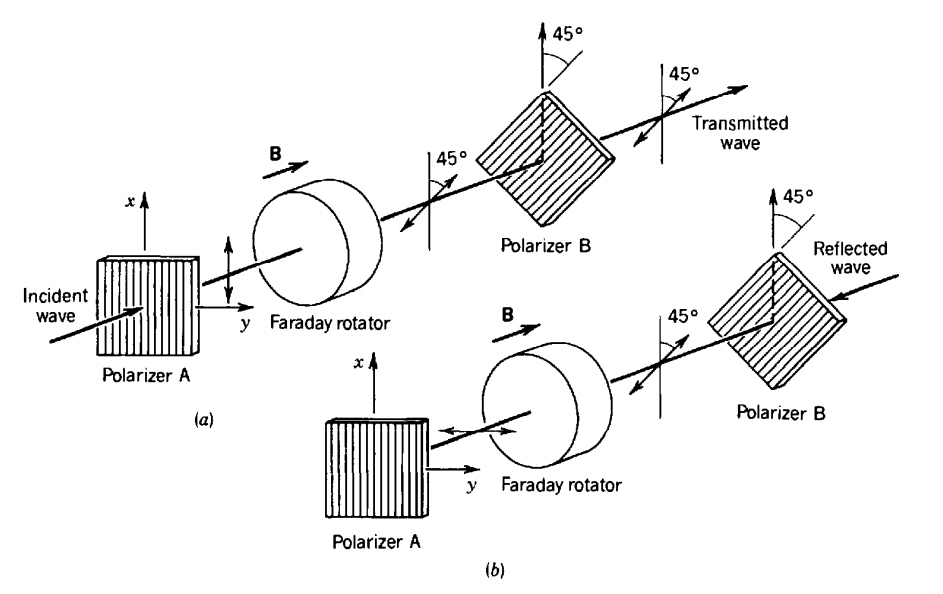
\includegraphics[width = 0.75\columnwidth]{Figures/Faraday-Insulator.png}
  \caption{Faraday insulator, taken from \cite{Saleh1991}. Light traveling from left to right is transmited while light propagating in the opposite direction is blocked by the polarizer $A$.}
  \label{fig:Faraday-insulator}
\end{figure}

At this point we can see that a common ingredient between devices which show a diode-like behaviour is some kind of internal structural asymmetry. In the case of the electric diode this asymmetry comes from the asymmetric distribution of charge carriers: electrons on the $n$-side, and holes in the $p$-side. In the case of the optical isolator the orientation of the magnetic field breaks the symmetry of the system.

This thesis is devoted to explore the possibility of designing nano devices that implement a \textit{diodic} or rectifying mechanism to allow an asymmetric transport of matter and energy. I decided to divide this thesis into two parts according to the context in which I look for asymmetric transport and particular objectives.

In the first part I work with quantum 1-dimensional scattering. The objective of this part of is to design scattering potentials that lead to transmission and reflection coefficients which differ for wave packets coming from the left or the right. I will refer to this kind of potential as an atom diode, since ideally I want a potential that acts as a one-way barrier for quantum particles. In doing so I will explore also properties of non-Hermitian Hamiltonians, which are necessary for asymmetric scattering. The content of this part will be organized in the following way. In Chapter \ref{Chapter1} I will give a brief introduction to scattering theory in 1 dimension to continue with an exposition of different asymmetric scattering devices. I will discuss how different symmetries of the scattering Hamiltonian pose restrictions on what kind of devices can be designed. In particular, non-Hermitian and non-local Hamiltonians are required to obtain asymmetric scattering. Next I will present some scattering potentials that are designed ad-hoc to obtain asymmetric devices and study their performance as a function of incident momenta. In Chapter \ref{Chapter2} I will focus on the mathematical properties of non-local and non-Hermitian Hamiltonians. I extend the concepts of parity, time reversal and PT symmetry (parity and time reversal combined together) to an extended set of symmetry transformations with group structure. When the Hamiltonian is invariant with respect to some of these transformations, the poles of the Hamiltonian are symmetric with respect to the imaginary axis of the complex plane. In Chapter \ref{Chapter3} I present a possible physical realization for an asymmetric scattering Hamiltonian in a quantum optics setup.

In the second part I study heat rectification in mesoscopic systems. The objective in this part is to design an analog device to the diode that allows one-way heat propagation. In Chapter \ref{Chapter4} I design a thermal diode composed of a chain of non-linear oscillators with a localized defect. In Chapter \ref{Chapter5} I design a thermal diode which can be implemented on a trapped ions setup. It consists on a chain of individually trapped ions with a graded profile of the trapping frequency. This setup seizes long range interactions, due to the Coulomb force, to increase rectification power. In Chapter \ref{Chapter6} I study the requirements for having heat rectification with a solvable model. It is generally accepted that non-linear interactions are needed in order to have rectification, since a system with non-linear interactions will have a temperature-dependent spectrum. I demonstrate, however that it is possible to have temperature dependent features in a linear system that lead to rectification.

In the last chapter of this thesis I outline the main results and state the conclusions.







% \section*{Introduction to part I}

% \subsection*{Basics of linear algebra}
%
% To understand the mathematics of quantum physics one has to be familiarized first with the concept of vector and Hilbert spaces. In the following I shall restrict myself to vector spaces over the field of complex numbers, since they are the kind of vector space used in quantum mechanics. A vector space $V$ is a non-empty set of elements called vectors with a sum operation that for every pair of vectors $\ket{a}$, $\ket{b}$ in $V$ gives another vector $\ket{c}$ of $V$. This sum operation has to be commmutative, associative, it has to have a zero element and last, every element of $V$ has one and only one inverse element.
%
% an inner product is an operation defined in a vector space, that for every pair of vectors gives a complex number
% %
% \begin{equation}
%   \braket{a}{b} = z \in \mathbb{C}
% \end{equation}
% %
%
% A Hilbert space is a vector space doted of an inner product where all Cauchy sequences converge to an element of the space. The last requirement is important for spaces of infinite dimensionality.
%
%
%
%
% POSTULATES OF QUANTUM MECHANICS
%
% In quantum mechanics a physical system is described with a Hilbert space $\mathcal{H}$ and the states of the system (if the system is isolated) are represented by the elements of this Hilbert space.
%
% The observables of quantum systems, \textit{i.e.}, every physical property of the system that can be experimentally measured, are represented by self-adjoint linear operators. The eigenvalues of an observable correspond to the set of possible outcomes of the measurement. The eigenvector related to the eigenvalue corresponds to the state of the system that yields the outcome.
%
% The most relevant observable in quantum mechanics is the energy operator, or Hamiltonian $H$, since it is the generator of the time evolution of the state system. The Schrodinger equation
% %
% \begin{equation}
%   i\hbar \frac{\partial}{\partial t} \ket{\psi} = H \ket{\psi}
% \end{equation}
% %
% dictates the evolution of the system state $\ket{\psi}$ through time. In general, the Hamiltonian can change with time but it will be asumed to be constant in this thesis. The hermicity of the Hamiltonian implies.
%
% \begin{itemize}
%   \item The norm of the state vector $\sqrt{\braket{\psi}{\psi}}$ is constant.
%
%   \item The energies of the system are real.
% \end{itemize}
%
%
% The fact that the norm is constant is very important for the probabilistic interpretation of quantum mechanics since it implies the conservation of probability. For any observable, the sum of the probabilities of all the eigenvalues should always eq ual to one, if the norm is not constant this will not happen.
%
% But what happens with dissipation? It has been described with density operators and master equations but it could also be described with non-hermitian Hamiltonians.
%
% Non hermitian Hamiltonians have been used to describe decay in physical systems in a phenomenological fashion \cite{Muga2004}.


% \section*{Introduction to part II}
%%
%
% \section*{Proposal of content}
%
% \begin{itemize}
%   \item PART I: Non-Hermitian Asymmetric Transmission Devices
%
%     \begin{itemize}
%       \item Chapter 1. \textbf{Asymmetric scattering by non-Hermitian potentials}.
%       This chapter is based in the following article:
%
%       \begin{itemize}
%         \item Asymmetric scattering by non-Hermitian potentials
%       \end{itemize}
%
%       \item Chapter 2. \textbf{Symmetries of non-hermitian potentials}.
%       This chapter is based in the following articles:
%
%       \begin{itemize}
%         \item Symmetries and invariants for non-Hermitian Hamiltonians
%         \item $S$-matrix pole symmetries for non-Hermitian scattering Hamiltonians
%         \item Symmetries of ($N \times N$) non-Hermitian Hamiltonian matrices
%       \end{itemize}
%
%       \item Chapter 3. \textbf{Physical Implementation of non-hermitian and non-local Hamiltonians}.
%       This chapter is based in the following article:
%
%       \begin{itemize}
%         \item Quantum-optical implementation of non-Hermitian potentials for asymmetric scattering.
%       \end{itemize}
%
%     \end{itemize}
%
%   \item PART II: Heat Rectification in mesoscopic devices/systems
%
%     \begin{itemize}
%       \item Chapter 4. \textbf{Heat Rectification with local impurities}.
%       This chapter is based in the following article:
%
%       \begin{itemize}
%         \item Local rectification of heat flux.
%       \end{itemize}
%
%       \item Chapter 5. \textbf{Heat Rectification in graded chains of trapped ions}.
%       This chapter is based in the following article:
%
%       \begin{itemize}
%         \item Asymmetric heat transport in ion crystals
%       \end{itemize}
%
%       \item Chapter 6. \textbf{Rectification in a minimal model}.
%       This chapter is based in the following article:
%
%       \begin{itemize}
%         \item Heat rectification with a minimal model of two harmonic oscillators
%       \end{itemize}
%
%     \end{itemize}
%
%   \item Conclusions
%
%   \item Appendices
%
%   \item Biliography
% \end{itemize}
